\documentclass{scrartcl}

\usepackage{german}
\usepackage[utf8]{inputenc}  %Umlaute
\usepackage[T1]{fontenc}     %Umlauttrennung
\usepackage{lmodern}         %modernes Schriftbild
\usepackage{amsmath}         %math Umgebungen
\usepackage{graphicx}
\usepackage{hyperref}
\usepackage{graphicx}
\usepackage{gensymb}
\usepackage{amssymb}
\usepackage{float}           %Positionierung von Tabellen und Abb

\title{Physikpraktikum für Naturwissenschaftler \\ Versuch: Schallwellen}
\author{Felix Burr, Johannes Spindler (Gruppe 13)}
\date{Durchgeführt am 25. Oktober 2018}


\begin{document}
\begin{titlepage}
  \begin{center}
    \vspace*{1cm}
    \LARGE
    Physikpraktikum für Naturwissenschaftler \\
    \vspace*{1cm}
    \Huge
    \textbf{Versuch: Schallwellen} \\
    \vspace*{0.3cm}
    \Large
    Durchgeführt am 25. Oktober 2018 \\
    Betreuer: Richard Waltrich \\
    \vspace*{2.5cm}
    Gruppe 13 \\
    Felix Burr: felix.burr@uni-ulm.de \\
    Johannes Spindler: johannes.spindler@uni-ulm.de \\
    \vfill 
  \end{center}
  Wir bestätigen hiermit, das Protokoll selbstständig erarbeitet zu haben und in genauer Kenntnis über dessen Inhalt zu sein. \\
  \vspace*{0.8cm}
  \\
  Felix Burr
  \hfill
  Johannes Spindler
\end{titlepage}
\pagebreak
\tableofcontents


\pagebreak

\section{Einleitung}
Schallwellen sind uns aus dem Alltag wohlbekannt. Als menschliche Stimme werden sie im Kehlkopf geformt, physikalisch betrachtet ist der Luftdruck hier die Größe, die sich zeitlich und örtlich periodisch ändert. Mit dem Ohr kann diese Druckänderung wahrgenommen und im Gehirn verarbeitet werden.

Die Entfernung eines Blitzeinschlags kann auch einfach abgeschätzt werden, wenn die Schallgeschwindigkeit in Luft bekannt ist: Ist der Einschlag einen Kilometer entfernt, verstreichen drei Sekunden zwischen Blitz und Donner.

Grund genug, sich dem interessanten Phänomen der Schallwellen zu widmen.
\section{Versuch 1: Schallgeschwindigkeiten in Gasen (Luft und $CO_{2}$)}
\subsection{Versuchsdurchführung}
Ziel des Versuches ist es, mithilfe eines Quincke'schen Resonanzrohres die Schallgeschwindigkeiten in Luft und $CO_{2}$ und daraus den Adiabatenexponenten in $CO_{2}$ zu berechnen.
\\

Der Versuchsaufbau sieht aus wie in Abbildung \ref{fig:Quincke}: Ein Lautsprecher ist an einen Frequenzgenerator angeschlossen und ist über einem oben offenen Glasrohr angebracht. Innerhalb des Glasrohrs befindet sich ein vertikal beweglicher Stempel mit einem Mikrofon. Das Mikrofon ist an ein Voltmeter angeschlossen. Am Rohr kann an einer Millimeter-Skala die Position des Stempels abgelesen werden.

\begin{figure}[h]
  \centering
    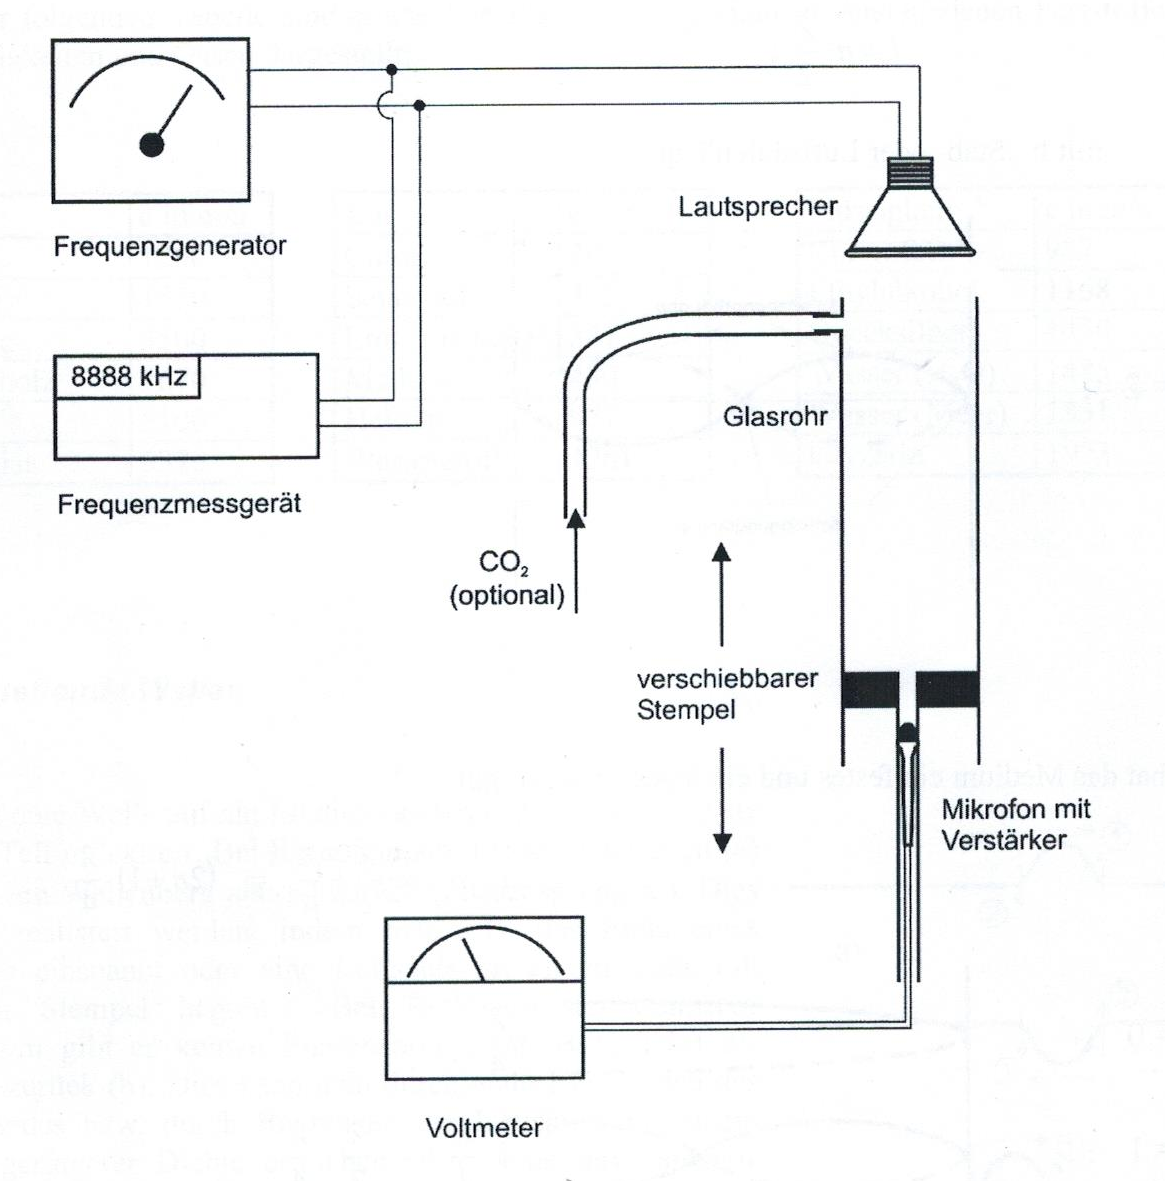
\includegraphics[scale=0.50]{Quincke.PNG}
  \caption{Quincke'sches Resonanzrohr (aus der Versuchsanleitung)}
  \label{fig:Quincke}
\end{figure}

Zuerst wird die tiefstmögliche Stempelposition $x_{0}$ gesucht, an der das Voltmeter maximal ausschlägt. An den Maximapositionen muss es sich um eine stehende Welle handeln. Eine Welle ist stehend, wenn die Schwingungsknoten sich zeitlich nicht bewegen.  Dann ist die Wellenreflexion deckungsgleich zur Welle, was bedeutet dass die Bäuche übereinander liegen und sich also verstärken. Da das Trägermedium (Gas in der Glasröhre) nach beiden Seiten begrenzt ist, gilt hier die folgende Bedingung für stehende Wellen:
\begin{align}
d = n  \cdot \frac{\lambda}{2}, n \in \mathbb{N}
\end{align}
Wenn $x_{0}$ gefunden ist, wird der Stempel bis zu einem Maximum an Position $x_{n}$ geschoben, die möglichst nahe am oberen Rohrende liegt. Dabei wird die Anzahl $n$ der zurückgelegten Intervalle zwischen Maxima gezählt. Der Abstand $d = x_{n} - x_{0}$ entspricht dann dem $n$-Fachen der halben Wellenlänge. Also kann aus Gleichung 1 die Wellenlänge $\lambda$ berechnet werden:
\begin{align}
\lambda = 2 \dfrac{d}{n} =  2 \dfrac{x_{n}-x_{0}}{n}
\end{align}
Die Wellenlänge und die eingestellte Frequenz $f$ führen zur Schallgeschwindigkeit $c$:
\begin{align}
c = \lambda f
\end{align}
Bei der Bestimmung der Schallgeschwindigkeit in $CO_{2}$ wird genauso vorgegangen, mit dem Unterschied, dass über einen seitlichen Anschluss am Glasrohr vor den Messungen $CO_{2}$ eingeleitet wird. Zwischen den Messungen muss immer wieder etwas $CO_{2}$ nachgefüllt werden um Verluste auszugleichen.

Nun wird die Zimmertemperatur gemessen, um die (temperaturabhängige) Dichte $\rho$ des $CO_{2}$ zu bestimmen:
\begin{align}
\rho & = \dfrac{\rho_{0}}{1 + \dfrac{\vartheta}{273,2 \degree C}} \\
\rho_{0} & = 1,9768 \dfrac{kg}{m^3}
\end{align}
Mit diesem Wert und dem gemessenen Umgebungsdruck $p$ erhält man schließlich den Adiabatenexponenten $\kappa$ von $CO_{2}$:
\begin{align}
\kappa = \dfrac{c^2 \cdot \rho}{p}
\end{align}
\newpage
\subsection{Messwerte und Ergebnisse}
\subsubsection{Im Medium Luft}
\begin{table}[h!]
\begin{tabular}{l|l|l|l|l|l|l|l}
Messung & $f$ {[}Hz{]} & $x_{0}$ [mm] & n & $x_{n}$ [mm] & $d$ [mm]   & $\lambda$ [m]      & $c$ [m/s]      \\
\hline
1       & 1666       & 43                & 3 & 350               & 307 & 0,205 & 341,0 \\
2       & 1666       & 39                & 3 & 350               & 311 & 0,207 & 345,4 \\
3       & 2000       & 30                & 3 & 288               & 258 & 0,172 & 344,0 \\
4       & 2000       & 28                & 3 & 287               & 259 & 0,173 & 345,3 \\
5       & 2333       & 27                & 4 & 321               & 294 & 0,147 & 343,0 \\
6       & 2333       & 27                & 4 & 322               & 295 & 0,148 & 344,1 \\
7       & 2666       & 27                & 5 & 349               & 322 & 0,129 & 343,4 \\
8       & 2666       & 28                & 5 & 349               & 321 & 0,128 & 342,3 \\
9       & 3000       & 27                & 6 & 373               & 346 & 0,115 & 346,0 \\
10      & 3000       & 27                & 6 & 372               & 345 & 0,115 & 345,0 \\
11      & 3333       & 33                & 6 & 350               & 317 & 0,106 & 352,2 \\
12      & 3333       & 34                & 6 & 343               & 309 & 0,103 & 343,3 \\
13      & 3666       & 40                & 6 & 322               & 282 & 0,094 & 344,6 \\
14      & 3666       & 42                & 6 & 323               & 281 & 0,094 & 343,4 \\
15      & 4000       & 47                & 7 & 352               & 305 & 0,087 & 348,6 \\
16      & 4000       & 46                & 7 & 350               & 304 & 0,087 & 347,4 \\
17      & 4333       & 17                & 8 & 338               & 321 & 0,080 & 347,7 \\
18      & 4333       & 16                & 8 & 340               & 324 & 0,081 & 351,0 \\
19      & 4666       & 27                & 8 & 321               & 294 & 0,074 & 343,0 \\
20      & 4666       & 26                & 8 & 324               & 298 & 0,075 & 347,6 \\
\hline
Mittelwert & & & & & & & 345,4
\end{tabular}
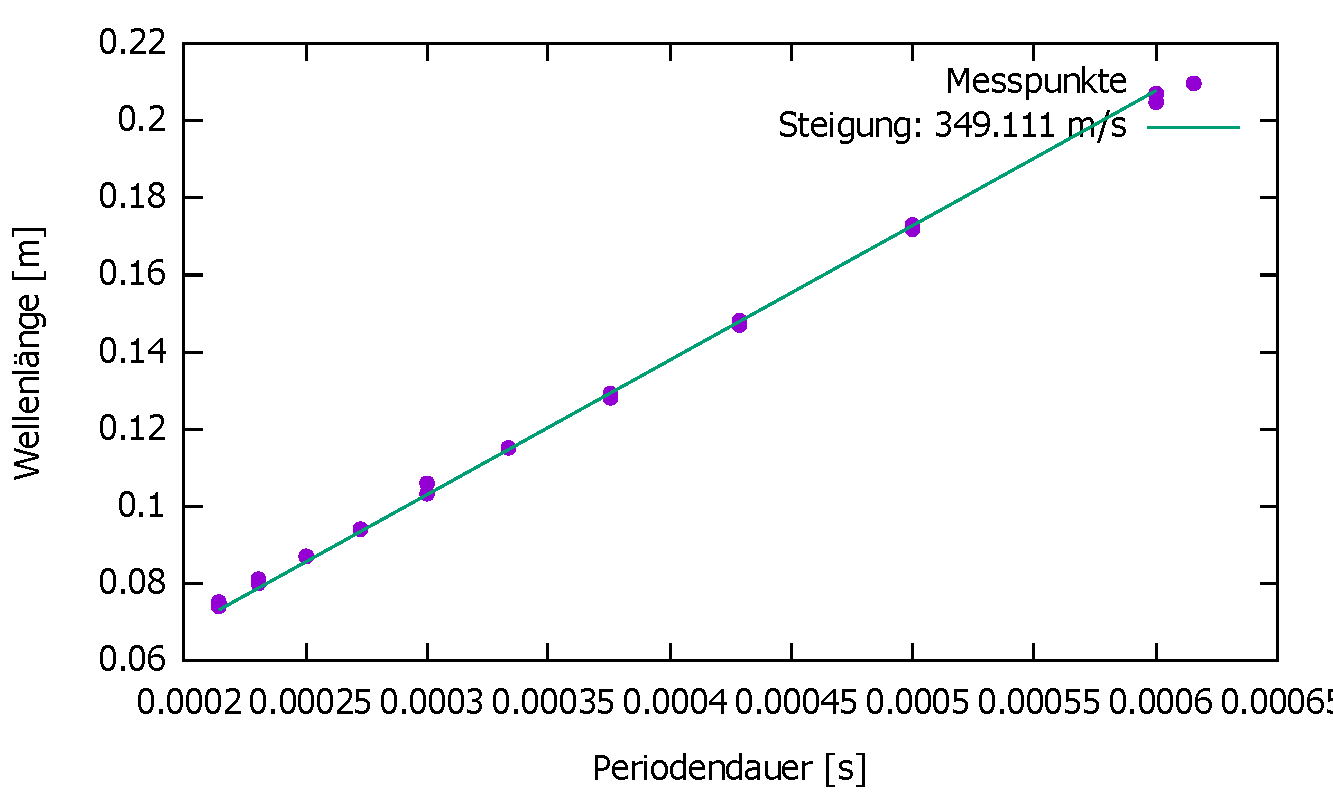
\includegraphics[width=1\textwidth]{linregV1_L.pdf}
\end{table}

\newpage
\subsubsection{Im Medium $CO_{2}$}
\begin{table}[h!]
\begin{tabular}{l|l|l|l|l|l|l|l}
Messung & $f$ {[}Hz{]} & $x_{0}$ [mm] & n & $x_{n}$ [mm] & $d$ [mm]   & $\lambda$ [m]      & $c$ [m/s]      \\
\hline
1       & 1666       & 43                & 3 & 295               & 252 & 0,168 & 279,9 \\
2       & 1666       & 49                & 3 & 297               & 248 & 0,165 & 275,4 \\
3       & 2000       & 48                & 4 & 330               & 282 & 0,141 & 282,0 \\
4       & 2000       & 56                & 4 & 330               & 274 & 0,137 & 274,0 \\
5       & 2333       & 68                & 5 & 361               & 293 & 0,117 & 273,4 \\
6       & 2333       & 69                & 5 & 362               & 293 & 0,117 & 273,4 \\
7       & 2666       & 78                & 5 & 335               & 257 & 0,103 & 274,1 \\
8       & 2666       & 68                & 5 & 330               & 262 & 0,105 & 279,4 \\
9       & 3000       & 29                & 6 & 315               & 286 & 0,095 & 286,0 \\
10      & 3000       & 32                & 6 & 313               & 281 & 0,093 & 281,0 \\
11      & 3333       & 20                & 7 & 304               & 284 & 0,081 & 270,4 \\
12      & 3333       & 18                & 7 & 306               & 288 & 0,082 & 274,3 \\
13      & 3666       &  0                & 9 & 331               & 331 & 0,074 & 269,7 \\
14      & 3666       & 27                & 9 & 364               & 337 & 0,075 & 274,5 \\
15      & 4000       & 42                & 9 & 350               & 308 & 0,068 & 273,8 \\
16      & 4000       & 50                & 9 & 360               & 310 & 0,069 & 275,6 \\
17      & 4333       & 33                & 10 & 345               & 312 & 0,062 & 270,4 \\
18      & 4333       & 32                & 10 & 349               & 317 & 0,063 & 274,7 \\
19      & 4666       & 11                & 11 & 331               & 320 & 0,058 & 271,5 \\
20      & 4666       & 10                & 11 & 332               & 322 & 0,059 & 273,2 \\
\hline
Mittelwert & & & & & & & 275,0
\end{tabular}
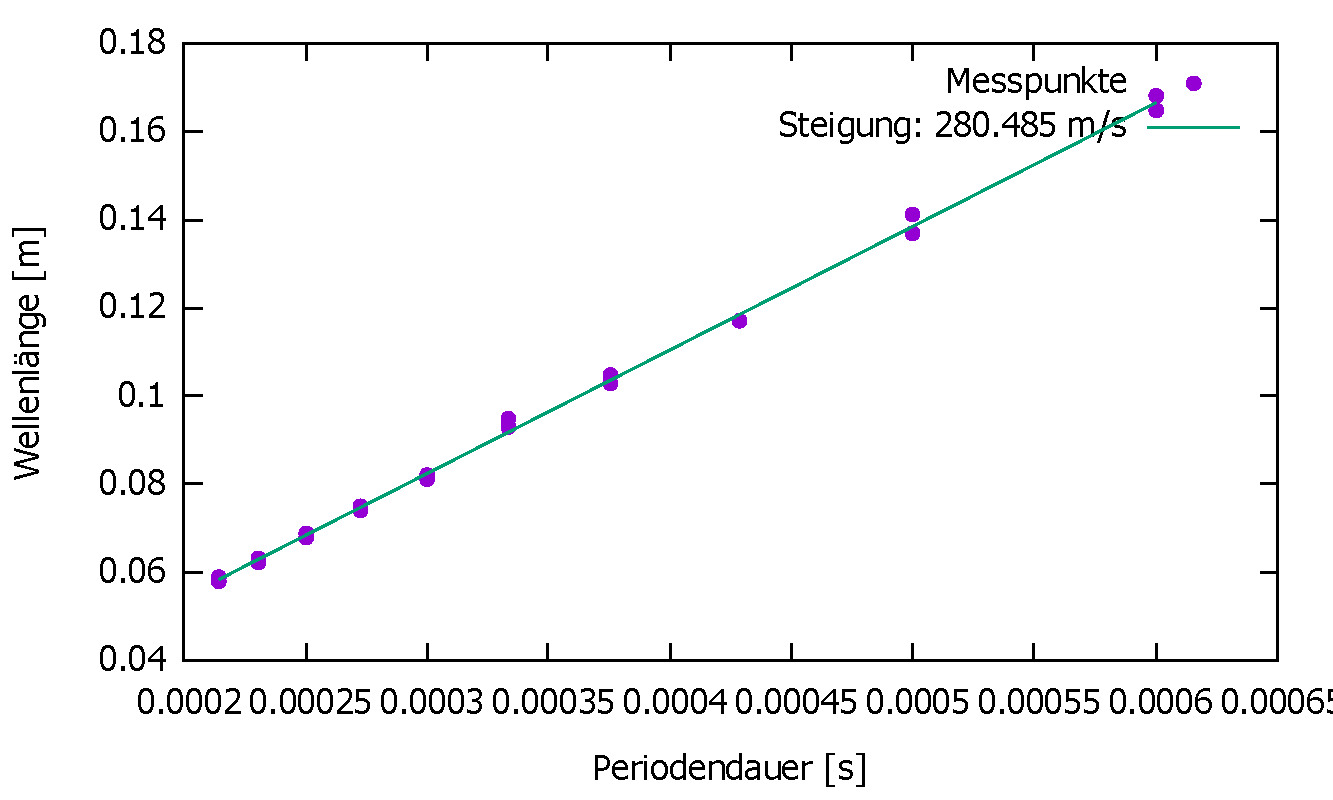
\includegraphics[width=1\textwidth]{linregV1_C.pdf}
\end{table}
Gemessene Raumtemperatur $\vartheta = 22,9\degree C$, daraus folgt 
\begin{align*}
\rho =  \dfrac{1,9768 \dfrac{kg}{m^3}}{1 + \dfrac{22,9\degree C}{273,2 \degree C}} = 1,8239 \dfrac{kg}{m^3}.
\end{align*}
Gemessener Luftdruck $p = 951 mBar = 95100 Pa$.
\begin{align*}
\kappa = \dfrac{c^2 \cdot \rho}{p} = \dfrac{(275,3 \dfrac{m}{s} \cdot 1,8239 \dfrac{kg}{m^3}}{95100 Pa} = 1,45 \dfrac{\dfrac{kg}{ms^2}}{Pa} = 1,45 \dfrac{\dfrac{N}{m^2}}{Pa} = 1,45
\end{align*}
\subsection{Fehlerrechnung}
\begin{align*}
\Delta d & = \left| \dfrac{\partial d}{\partial x_{n}} \right| \Delta x_{n} + \left| \dfrac{\partial d}{\partial x_{0}} \right| \Delta x_{0} = \left| 1 \right| \Delta x_{n} + \left| -1 \right| \Delta x_{0} = \Delta x_{n} + \Delta x_{0} \\
\Delta \lambda & = \left| \dfrac{\partial \lambda}{\partial d} \right| \Delta d + \left| \dfrac{\partial \lambda}{\partial n} \right| \Delta n = \left| \dfrac{2}{n} \right| (\Delta x_{n} + \Delta x_{0}) + \left| - \dfrac{2d}{n^2} \right| \Delta n \\
& = \dfrac{2}{n} \Delta x_{n} + \dfrac{2}{n} \Delta x_{0} + \dfrac{2d}{n^2} \Delta n = \dfrac{2}{n} (\Delta x_{n} + \Delta x_{0} + \dfrac{d}{n} \Delta n) \\
& = \dfrac{2}{n} (\Delta x_{n} + \Delta x_{0} + \dfrac{x_{n} - x_{0}}{n} \Delta n)\\
\Delta c & = \left| \dfrac{\partial c}{\partial \lambda} \right| \Delta \lambda = \left| f \right| \Delta \lambda = \dfrac{2f}{n} (\Delta x_{n} + \Delta x_{0} + \dfrac{x_{n} - x_{0}}{n} \Delta n)
\end{align*}
\subsection{Ergebnisdiskussion}
In Versuch 2 wurde die Schallgeschwindigkeit in Luft bei der gemessenen Raumtemperatur mit Gleichung 11 berechnet, dies ergab $344 \dfrac{m}{s}$.
Für die Geschwindigkeit in $CO_{2}$ kann laut Anleitung $266 \dfrac{m}{s}$ als Vergleichswert herangezogen werden.
Man erkennt, dass die Messung in Luft um 0,4 \% abweicht, während die Messung in $CO_{2}$ mit 3,5 \% stärker abweicht. Der Grund hierfür ist, dass beim Verschieben des Stempels nach oben und anschließendem Zurückschieben nach unten ein Unterdruck in der Glasröhre entsteht und dadurch Luft angesaugt wird. Außerdem verschließt der Stempel den unteren Rohrausgang nicht völlig luftdicht, weshalb hier etwas $CO_{2}$ ausfließen kann.
\section{Versuch 2: Schallgeschwindigkeit in einem Messingstab}
\subsection{Versuchsdurchführung}
Mit einem Kundt'schen Staubrohr wird die Schallgeschwindigkeit $c$ in einem Messingstab und daraus das Elastizitätsmodul $E$ des Stabs berechnet.

Beim Kundt'schen Staubrohr (siehe Abbildung \ref{fig:Kundt}) handelt es sich um ein mit etwas Korkmehl gefülltes Glasrohr, das auf einer Seite mit einem beweglichen Stempel geschlossen ist und in dessen andere Seite ein Messingstab ragt. Der Stab ist an zwei Punkten über dem Tisch eingespannt.

\begin{figure}[h]
  \centering
    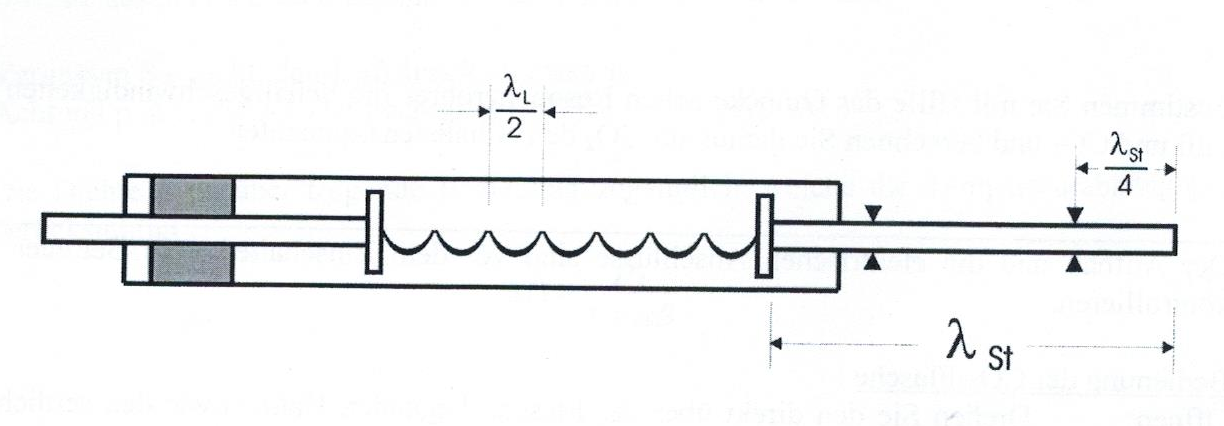
\includegraphics[scale=0.50]{Kundt.PNG}
  \caption{Kundt'sches Staubrohr (aus der Versuchsanleitung)}
  \label{fig:Kundt}
\end{figure}

Der Stempel wird nun so eingestellt, dass für die Länge $l$ und die Wellenlänge $\lambda$ der Luftsäule zwischen Ende des Messingstabs und Stempel gilt:
\begin{align}
l = n  \cdot \frac{\lambda}{2}, n \in N
\end{align}
Selbiges muss für den Messingstab gelten, wobei $l$ dann der Abstand zwischen den Einspannpunkten und $\lambda$ die Länge und gleichzeitig Wellenlänge des Stabs ist. Also werden die Einspannpunkte bei einer viertel Stablänge und bei einer dreiviertel Stablänge gewählt.
Wird mit einem ethanolbefeuchteten Tuch am Stab gerieben, schwingt dieser mit der Frequenz $f = f_{Stab} = f_{Luft}$, die sich auf die Luftsäule überträgt. Mit 
\begin{align}
f = \dfrac{c}{\lambda}
\end{align}
ergibt sich folgender Zusammenhang zwischen Stab und Luft:
\begin{align}
\dfrac{c_{Stab}}{\lambda_{Stab}} = \dfrac{c_{Luft}}{\lambda_{Luft}}
\end{align}
Durch die Schwingung der Luftsäule formt der Staub im Rohr ein Wellenmuster, wobei der Abstand zweier Wellenbäuche gerade $\lambda_{L} / 2$ beträgt. 
Es wird in mehreren Messungen also der Stab zum Schwingen angeregt, dann wird die Anzahl $b$ der sichtbaren Halbwellenlängen im Staub (das Intervall zwischen zwei Wellenbäuchen ist eine Halbwellenlänge) und der Abstand $x$ zwischen erstem und letztem erkennbaren Wellenbauch ermittelt und $\lambda_{L}$ berechnet:
\begin{align}
\dfrac{\lambda_{L}}{2} = \dfrac{x}{b}
\end{align}
$\lambda_{S}$ entspricht gerade der Länge des Stabs und $c_{L}$ erhält man, abhängig von der Raumtemperatur $\vartheta$ durch
\begin{align}
c_{L} = c_{L, 0} & \cdot \sqrt{1+\dfrac{\vartheta}{273,2 \degree C}} \\
c_{L, 0} & = 331 \dfrac{m}{s}
\end{align}
Damit sind alle Größen bekannt, um $c_{S}$ mit (6) zu berechnen. Für das Elastizitätsmodul gilt dann:
\begin{align}
c_{S} = \sqrt{\dfrac{E}{\rho}} \\
E = c_{S}^2 \rho
\end{align}
Die Temperaturabhängigkeit der Dichte $\rho$ der Messinglegierung kann bei Metallen vernachlässigt werden.
\subsection{Messwerte und Ergebnisse}
\begin{table}[h]
\begin{tabular}{l|l|l|l}
Messung & $b$ & $x$ [m] & $\lambda_{L}$ [m]      \\
\hline
1       & 4            & 0,32    & 0,160 \\
2       & 6            & 0,39    & 0,130 \\
3       & 4            & 0,31    & 0,155 \\
4       & 4            & 0,31    & 0,155 \\
5       & 4            & 0,31    & 0,155 \\
6       & 3            & 0,26    & 0,173 \\
7       & 4            & 0,31    & 0,155 \\
8       & 3            & 0,24    & 0,160 \\
\hline
Mittelwert & & & 0,155
\end{tabular}
\end{table}
Gemessene Raumtemperatur $\vartheta = 22,9\degree C$,

daraus folgt $c_{L} = 331 \dfrac{m}{s} \cdot \sqrt{1+\dfrac{22,9\degree C}{273,2 \degree C}} = 344 \dfrac{m}{s}$.

Stablänge $\lambda_{S} = 1,60m$.

Also $c_{S} = \dfrac{c_{L}}{\lambda_{L}} \cdot \lambda_{S} = \dfrac{344\dfrac{m}{s}}{0,155m} \cdot 1,60m = 3550 \dfrac{m}{s}$

Mit dem Wert $\rho = 8,44 \dfrac{g}{cm^3} = 8,44 \dfrac{10^{-3} kg}{10^{-6} m^3} = 8440 \dfrac{kg}{m^3}$ aus der Versuchsanleitung \\ kann das Elastizitätsmodul $E$ berechnet werden:
\begin{align*}
E = c_{S}^2 \rho = 3550^2 \cdot 8440 \cdot \dfrac{m^2}{s^2} \dfrac{kg}{m^3} = 1,06 \cdot 10^{11} \dfrac{kg}{ms^2} = 1,06 \cdot 10^{11} \dfrac{N}{m^2} = 106 GPa
\end{align*}

\subsection{Ergebnisdiskussion}
Der hier bestimmte Wert $c_{S}$ für die Schallgeschwindigkeit in Messing überschreitet den Literaturwert  von 3530 m/s auf der Versuchsanleitung um 0,6 \%. Das bedeutet, die Messungen 3, 4, 5, 7, die dem Mittelwert für $c_{L}$ entsprechen, waren am genauesten. Fehler bei den anderen Messungen lassen sich durch schlechter ausgeprägte Wellenmuster im Staub und ungenaues Ablesen erklären. 

Der berechnete Wert für $E$ unterschreitet den Literaturwerts von 110 GPa um 3,6 \%. Diese Abweichung ist wahrscheinlich auf das Vernachlässigen der Temperaturabhängigkeit der Dichte $\rho$ zurückzuführen.


\section{Versuch 3: Direkte Messung der Schallgeschwindigkeit in Luft}
\subsection{Versuchsdurchführung}
In diesem Versuch wird per Frequenzgenerator eine Frequenz erzeugt, welche am Lautsprecher ein akustisches Signal erzeugt. Ein Mikrofon auf einer Schiene registriert das Signal. Beide Signale - die des Frequenzgenerators und die des Mikrophons - werden mittels Oszilloskop angezeigt. 
Versetzt man nun das Mikrofon, sieht man am Oszilloskop wie sich die Welle verschiebt.
Mittels Gleichung (3) kann man die Schallgeschwindigkeit ermitteln
\subsection{Messwerte und Ergebnisse}
\begin{table}[H]
\begin{tabular}{l|l|l|l|l}
Messung & Distanz $[cm]$ & Anzahl Perioden & Frequenz $[hz]$ & Wellenlänge $[cm]$ \\ \hline
1       & 24.0          & 4 & 6000 & 6.00\\
2       & 22.1          & 4 & 6500 & 5.53\\
3       & 25.1          & 5 & 7000 & 5.02\\
4       & 21.1          & 4 & 7500 & 5.23\\
5       & 18.2          & 4 & 8000 & 4.55\\
6       & 16.8          & 4 & 8500 & 4.20\\
7       & 20.7          & 5 & 9000 & 4.14\\
\end{tabular}
\end{table}
Mit (3) resultiert, dass die Schallgeschwindigkeit im Mittel $365$ Meter pro Sekunde beträgt.
\subsection{Ergebnisdiskussion}
Der hier Bestimmte Wert für die Schallgeschwindigkeit in Luft weicht im  Vergleich mit dem Literaturwert von $343 \frac{m}{s}$ um ganze $22\frac{m}{s}$ ab. Dies wird vor allem an Messfehlern beim Ablesen liegen.
\section{Versuch 4: Messung der Schallgeschwindigkeit mittels Frequenzanalyse}
\subsection{Versuchsdurchführung}
Wie in Versuch 2 beschrieben, wird hier ein Messingstab in Schwingung versetzt. Dies wird mit einem Mikrofon gemessen und im Oszilloskop mittels dem "Fast Fourier Transformation" Modus visualisiert. Zu sehen ist nun das Frequenzspektrum des Signals. Wir lesen die Frequenz der einzelnen dargestellten Peaks ab und erhalten dadurch die Frequenzen der verschiedenen Schwingungsmoden. Durch Gleichung (13) kann die Schallgeschwindigkeit ermittelt werden.\begin{align}
V_{Schall} = f \cdot d_{Knoten}
\end{align}
\subsection{Messwerte und Ergebnisse}
\begin{table}[H]
\begin{tabular}{l|l}
Peak Nummer &	Frequenz $[hz]$\\ \hline
1			&	2200\\
2			&	4400\\
3			&	6600\\
4			&	8800\\
5			&	111000\\
6			&	132000\\
\end{tabular}
\end{table}
Skizze der n-ten Harmonischen:
\begin{figure}[H]
  \centering
    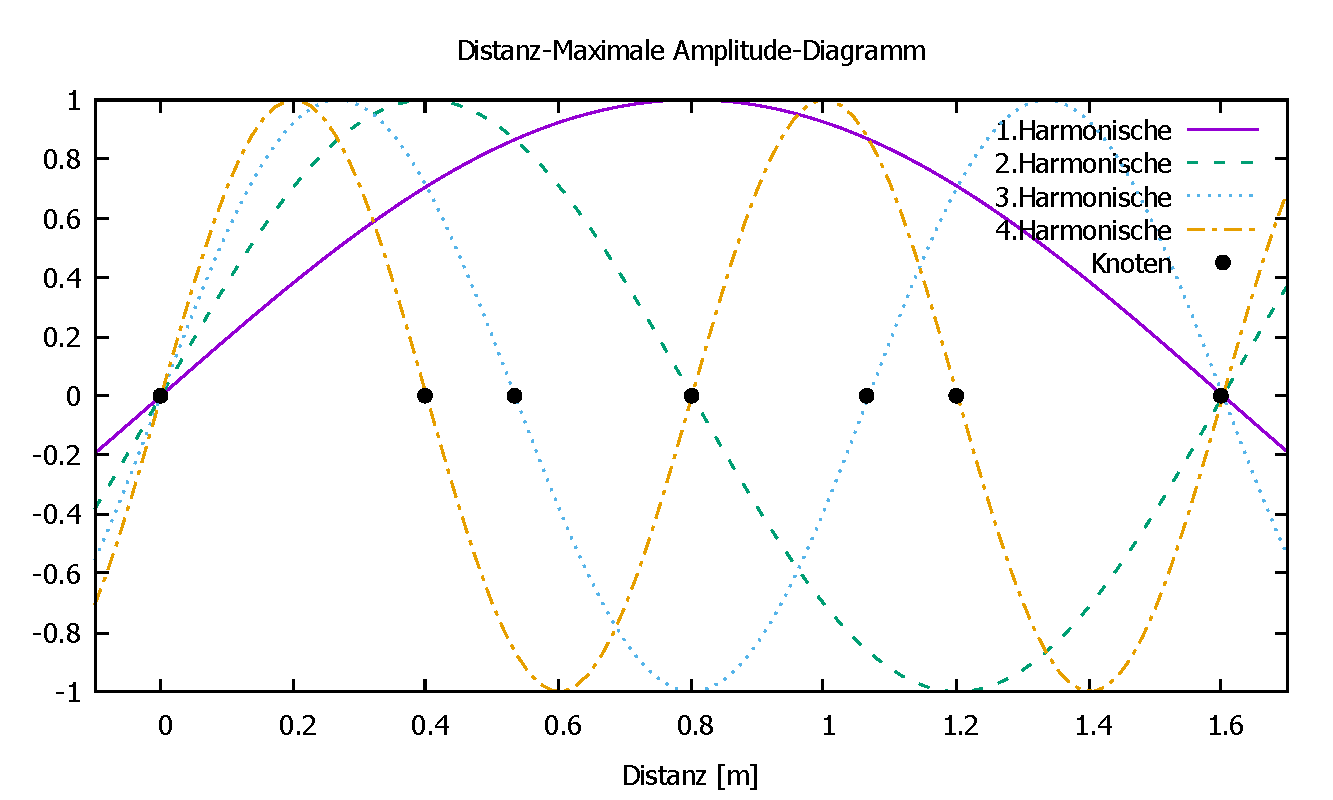
\includegraphics[width=1\textwidth]{Versuch4_skizze.pdf}
  
  \label{fig:Diagramm}
\end{figure}
\begin{table}[H]
Auswertung der Schallgeschwindigkeit mithilfe von Gleichung (13):
\begin{tabular}{l|l|l|l}
n-te Harmonische &	Distanz $[m]$ & Frequenz $[hz]$&Schallgeschwindigkeit $[\frac{m}{s}]$\\ \hline
1			&	1.6		&	2200	&	 3520\\
2			&	0.8		&	4400	&	 3520\\
3			&	0.533	& 	6600	&	3520\\
4			&	0.4		& 	8800	&	3520\\

\end{tabular}
\end{table}
\subsection{Ergebnisdiskussion}
Die Schallgeschwindigkeit in Messing beträgt nach diesen Messungen $3520\frac{m}{s}$. Somit unterschreitet dies den Literaturwert von $3530\frac{m}{s}$ um $0.3\%$.

\end{document}

